\documentclass{article}

\usepackage{graphicx}

\usepackage{hyperref}
\hypersetup{colorlinks=true,
			linkcolor=blue,
			filecolor=magenta,
			urlcolor=cyan,
}
\urlstyle{same}

\usepackage{booktabs}
\usepackage{tabularx}

\title{SE 3XA3: Development Plan\\Staroids}

\author{Team 20, Staroids
		\\ Moziah San Vicente, 400091284, sanvicem
		\\ Eoin Lynagh, 400067675, lynaghe
		\\ Jason Nagy, 400055130, nagyj2
}

\date{Friday September 28, 2018}

%\input{../Comments}

\begin{document}

\begin{table}[hp]
\caption{Revision History} \label{TblRevisionHistory}
\begin{tabularx}{\textwidth}{llX}
\toprule
\textbf{Date} & \textbf{Developer(s)} & \textbf{Change}\\
\midrule
Sept 21 & Eoin, Jason, Moziah & Added questions to be answered\\
Sept 23 & Jason & Added Communication Plan and Team Member Roles content\\
Sept 23 & Eoin & Added Coding Style content\\
Sept 23 & Jason & Added Git Workflow content\\
Sept 23 & Moziah & Added Technology content and Temporary Excel Gantt Chart\\
\bottomrule
\end{tabularx}
\end{table}

\newpage

\maketitle

Put your introductory blurb here.

\section{Team Meeting Plan}
Eoin
When?Where?Frequency?Roles?Rules for agendas?Upcoming milestones?Discuss problems?

Meetings Monday 5:30 (After 3BB4)

Agendas:
Form - Meeting Minutes
*Meeting Minutes obey Harvard guidelines
Chair - Jason/ Wallace
Scribe - Eoin

\section{Team Communication Plan}
Most work related jobs and tasks will be discussed through Facebook Messenger. The aformentioned discussion includes assigning work, talking about current issues, discussing what is next and how implementations should be done. Facebook Messenger will be used in addition to the scheduled meetings. The meetings will be about larger issues while Facebook Messenger will have simpler issues. If someone is unable to use Facebook Messenger for whatever reason, email can also be used for casual work discussion. Some examples of issues that are Facebook Messenger worthy are bugs in the program, code portions where the coder is unsure how to solve a problem, letting the team know what someone is currently working on.\\
For more time critical issues, the phone is to be used. It can be through text or call, but call is preferred because it allows for synchronous communication. Some example issues worth of phone communication include questions for work that are due soon and application crashing bugs, should they occur.\\
The members of Staroids have all exchanged phone and Facebook information.\\

\section{Team Member Roles}
The leader of Staroids will be Jason. As leader, he is responsible for organizing meetings and giving deadlines.\\
The scribe of Staroids will be Eoin. Eoin is in charge of meeting agendas and ensuring meeting documents are current and accurate. He is also responsible for assembling the meeting agendas from information from everyone.\\
The technology expert and submitter will be Moziah. Moziah is responsible for researching and implementing new technologies and tools to be used in the project while also ensuring that the Git repo is maintained properly. Moziah will also ensure the final versions of files are properly tagged.\\
As a group, Staroid members will collectively discuss and decide what the next tasks to complete are and who shall be assigned which parts, depending on why has what relevant skills.

\section{Git Workflow Plan}
Staroids has decided to use branching for this project. All Staroid memebers will have their own personal branches that will be periodically merged with the master. If any one member needs help from another, they can simply switch to their branch and then switch back once the issue has been resolved. Major versions will be based on milestones and minor versions will not be used. Milestones will both be project deliverables as well as group decided features. Another technology that is planned to be used is the Atom text editor's "Tele-type" functionality. This allows two members to simultaneously work on the same file from different computers. The main use of this tool will be for helping each other with problematic pieces of code.\\

labels - to be researched

\section{Proof of Concept Demonstration Plan}
All
research - look to slides

\section{Technology}
%JavaScript - Canvas
%HTML5
%Case based?
%LaTeX (pdflatex)
\subsection{Programming Language}
The programming language we are choosing to use for this project is JavaScript. Since JavaScript is a web developing language, we will be able to run our game on websites, which is a very big upside because it will be able to reach many more people than if it had to be downloaded. Also this makes it easier to play since no setup is required for the user, just typing in the web address or opening up the html file. Next, the original program that we are basing this re-implementation on was also written in JavaScript so we have a guide to look at when we are re-developing the project. As well another big proponent of us wanting to the develop the game in JavaScript, is that throughout our time in the Software Engineering program at McMaster University we haven’t yet got to do any web development projects, so this was a great opportunity to get some more experience in that for our team.
\subsection{IDE}
The IDE that we are going to use for our project development is Atom. Atom is one of the most widely used IDE’s for coding in a broad array of languages not just JavaScript, but even so, it is still rated a top five JavaScript IDE according to \url{https://jaxenter.com/top-5-javascript-ide-146609.html}. The other good features about this IDE that are really useful for our project and why we chose it are it’s git integration, as well as the ability to work on the same files together on different computers using its portal feature.
\subsection{Testing Framework}
The testing Framework we are going to use is a combination of two Frameworks called Mocha(Testing Framework) and Chai(Assertion Library). This is one of the most widely used JavaScript testing frameworks, and has a built in integration with our IDE Atom, to make testing as convenient and straightforward as possible for us.
\subsection{Document generation}
All of our documentation will be written in Latex, as specified in the course outline, and will then have a pdf form generated from that as also specified. The only exception to this will be for the documentation of our code, where we would like to use JsDoc to autogenerate the pdf documentation based on our comments. This is because it is a popular and widely used documentation tool for JavaScript, and has many tutorials and lots of info online to help us learn how to use it, like this for example \url{https://milmazz.uno/article/2014/08/27/how-to-document-your-javascript-code/}.
%https://medium.com/4thought-studios/documenting-javascript-projects-f72429da2eea




\section{Coding Style}
Eoin
\subsection{File Names}
File names will be written using camel case, and will use a descriptive title. For example, the title of this document is styleGuidelines.
\subsection{Variable Names}
Variable names will be written using camel case, and will be written as follows baseAttributeDescriptor, so for example, a variable representing the velocity of a ball would be named velocityBall.
\subsection{Javascript}
Javascript code will be written to follow the \href{https://google.github.io/styleguide/jsguide.html}{Google Javascript Style Guide}, which details coding standards for source code in JavaScript. However, the style of Variable/File names is described above, and may not follow the Google Style guide.
file names - camel case
variable names - camel case, [base attribute][descriptor]
follow https://google.github.io/styleguide/jsguide.html

\section{Project Schedule}
%Provide a pointer to your Gantt Chart.
\begin{center}
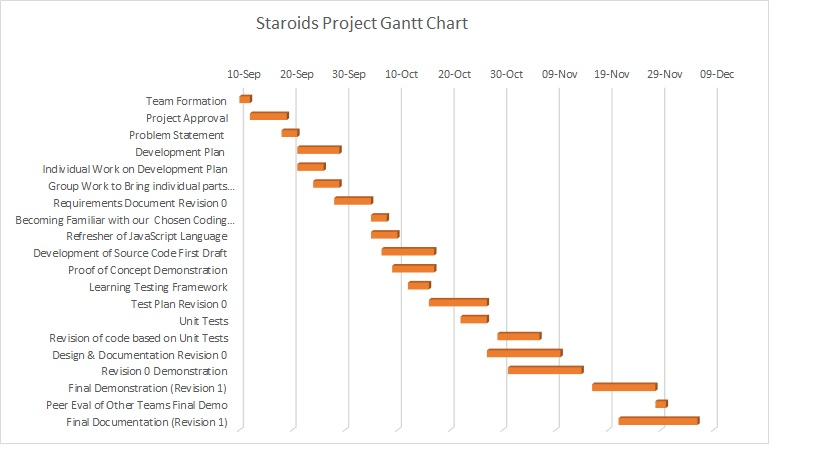
\includegraphics[scale=1]{gantt.jpg}
\end{center}


\section{Project Review}

- not actually completed

\end{document}
